% RPL-ClusterIDS — Computer Networks (Elsevier) preprint.
% Build:
%   pdflatex main && bibtex main && pdflatex main && pdflatex main
\documentclass[preprint,12pt,number]{elsarticle}

\usepackage{lmodern}
\usepackage[english]{babel}
\IfFileExists{microtype.sty}{%
  \usepackage{microtype}%
  \microtypesetup{nopatch={verbatim}}%
}{}
\usepackage{tikz}
\usetikzlibrary{arrows.meta,positioning,shapes.geometric}
\usepackage{pgfplots}
\pgfplotsset{compat=1.18}
\usetikzlibrary{pgfplots.statistics}
\IfFileExists{booktabs.sty}{\usepackage{booktabs}}{%
  \providecommand{\toprule}{\hline}%
  \providecommand{\midrule}{\hline}%
  \providecommand{\bottomrule}{\hline}%
}
\usepackage{amsmath,amssymb}
\IfFileExists{caption.sty}{%
  \usepackage{caption}%
  \captionsetup{font=small,labelfont=bf}%
}{}
\usepackage{tabularx}
\usepackage{array}
\usepackage{multirow}
\usepackage{adjustbox}
\usepackage{url}
\usepackage[hidelinks,bookmarksopen=true]{hyperref}

\graphicspath{{Figures/}}
% RPL-ClusterIDS — result-status markers. Pilot campaign (3 seeds).
\newcommand{\CaptionFigStatusNote}{(pilot campaign; preliminary only)}
\newcommand{\TableStatusNote}{(pilot results; preliminary only)}

% English figure captions for RPL-ClusterIDS (11-figure plan).

\newcommand{\CaptionFigOne}{%
  Conceptual architecture of RPL-ClusterIDS over an RPL DODAG. Member nodes execute lightweight rules and local anomaly scores (LAS); cluster heads aggregate evidence and run hybrid detection; sparse inter-cluster summaries bound control traffic. The border router optionally fuses cluster-level alerts.%
}

\newcommand{\CaptionFigTwo}{%
  Logical cluster overlay on a sample RPL DODAG. Cluster membership (dashed ovals) is decoupled from routing parents (solid arrows). Cluster heads sit on stable, energy-rich anchors while members report compact LAS summaries upward.%
}

\newcommand{\CaptionFigThree}{%
  Context-adaptive policy weights $(w_e,w_s,w_t,w_d)$ and operating-mode thresholds as a function of mean normalized residual energy (NRE) and dominant traffic-priority class. Higher $C3$ share increases monitoring depth; low NRE shifts the policy toward \textsc{Eco}.%
}

\newcommand{\CaptionFigFour}{%
  Detection rate across five RPL attack scenarios (50-node grid, \textsc{Balanced} mode, pilot campaign). RPL-ClusterIDS is compared with centralized rules (B1); B2 and B3 are pending full campaign evaluation.%
}

\newcommand{\CaptionFigFive}{%
  Mean detection latency from attack onset to confirmed cluster alert. Localized rank and selective-forwarding attacks are contained within one cluster; wormhole campaigns require inter-cluster corroboration and exhibit higher latency. $^\dag$B1 latency values reflect false-positive alert timing (0\% detection rate).%
}

\newcommand{\CaptionFigSix}{%
  False-positive rate stratified by traffic-priority class ($C0$--$C3$) in the mixed campaign scenario. B1 and RPL-ClusterIDS exhibit identical FPR in the pilot campaign; B2 and B3 pending evaluation.%
}

\newcommand{\CaptionFigSeven}{%
  Additional Energest-reported energy overhead on member and cluster-head nodes relative to a no-IDS baseline. \textsc{Eco} mode reduces member duty by disabling rules R3--R4 and deferring CH verification at heads.%
}

\newcommand{\CaptionFigEight}{%
  Alert and IDS control-packet overhead (packets per hour) at 50 nodes (pilot campaign; values beyond 50 nodes are design-target projections assuming sublinear scaling). RPL-ClusterIDS scales sublinearly because members signal only their cluster head and heads gate inter-cluster summaries.%
}

\newcommand{\CaptionFigNine}{%
  Cluster stability proxy: mean cluster-head tenure and reclustering frequency versus mean NRE. As energy drains, clusters merge and $\Delta_c$ lengthens to preserve lifetime.%
}

\newcommand{\CaptionFigTen}{%
  Temporal stratification of detection rate over the mixed attack campaign (stabilization, attack injection, recovery). RPL-ClusterIDS maintains sensitivity on $C3$ flows during the attack phase while \textsc{Eco} mode throttles non-critical checks during recovery.%
}

\newcommand{\CaptionFigEleven}{%
  Operating-mode sensitivity (\textsc{Full}, \textsc{Balanced}, \textsc{Eco}) for mixed-campaign detection rate, false-positive rate, and member CPU overhead. The policy exposes an explicit security-lifetime trade-off. DR and FPR share the left axis; CPU overhead is plotted on the right axis for readability.%
}

\hyphenation{RPL-ClusterIDS Contiki-NG Cooja DODAG}

\providecommand{\IEEEPARstart}[2]{\textbf{#1}#2}
\newcommand{\RPLClusterIDS}{RPL-ClusterIDS}
\newcommand{\RPLClusterIDSTag}{\texttt{RPL\_ClusterIDS}}

\journal{Computer Networks}

\begin{document}

\begin{frontmatter}

\title{RPL-ClusterIDS: A Clustering-Based, Energy-Aware and Context-Adaptive\\Distributed Intrusion Detection System for RPL in Resource-Constrained IoT Networks}

\author[univ]{Madani Belacel}
\cormark[1]
\ead{madani.belacel@univ-mosta.dz}

\affiliation[univ]{organization={Abdelhamid Ibn Badis University of Mostaganem},
            addressline={Mostaganem},
            city={Mostaganem},
            country={Algeria}}

\cortext[1]{Corresponding author}

\begin{highlights}
\item Hierarchical distributed IDS using energy-aware clusters for RPL-based IoT networks.
\item Cluster heads run two-stage threshold verification; members perform ultra-light rule screening.
\item Context-adaptive three-mode policy trades detection depth against network lifetime.
\item Cooja pilot campaign (3 seeds, 5 attack scenarios): 80.6\% DR, 0.50\% FPR, 5--7\% CPU overhead.
\item Full reproducibility package: firmware, campaign scripts, parsed datasets, and analysis pipeline.
\end{highlights}

\begin{abstract}
The Routing Protocol for Low-Power and Lossy Networks (RPL) underpins large-scale Internet of Things (IoT) deployments, yet its open control plane exposes constrained nodes to internal attacks such as rank manipulation, selective forwarding, wormhole tunneling, and DAO flooding.
Existing intrusion detection systems (IDS) for RPL often depend on a centralized border router, generate excessive peer-to-peer alerts in flat distributed designs, or ignore residual energy and traffic criticality.
This paper introduces RPL-ClusterIDS, a clustering-based hierarchical distributed IDS that organizes detection around dynamically formed, energy-aware clusters shaped by normalized residual energy, topological stability, and traffic-priority class.
Ordinary members execute ultra-lightweight rules and report compact local anomaly scores, while cluster heads perform rule-based two-stage threshold verification under a context-adaptive policy that modulates cluster granularity and monitoring depth.
The system is implemented in Contiki-NG and evaluated through a Cooja pilot campaign (21 seeds for the CLUSTERIDS variant, 3 seeds for the ablation study; 5 attack scenarios on a 50-node grid).
In this pilot campaign, RPL-ClusterIDS reached 80.6\% campaign-level detection rate\footnote{Campaign-level detection rate is defined as at least one confirmed alert during an attack period.} (95.1\% on individual attack scenarios) with 0.50\% false-positive rate and 5--7\% CPU overhead, while the B1 baseline remained at 0\% detection rate. Per-interval detection rate averaged 1.1\% across modes (see Fig.~\ref{fig:mode-sensitivity}). These findings should be interpreted as promising preliminary evidence rather than definitive performance claims.
The full artifact package, including firmware, campaign scripts, parsed datasets, and analysis pipeline, is publicly available at: \url{https://github.com/madani-belacel/IDS-IOT}

\end{abstract}

\begin{keyword}
RPL \sep IoT \sep intrusion detection \sep clustering \sep energy-aware security \sep context adaptation \sep distributed detection \sep Contiki-NG
\end{keyword}

\end{frontmatter}

\section{Introduction}
\label{sec:intro}

\IEEEPARstart{L}{ow-power} wireless IoT networks increasingly rely on the Routing Protocol for Low-Power and Lossy Networks (RPL) to build IPv6 connectivity over lossy links and duty-cycled radios~\cite{rfc6550,baronti2007}.
RPL organizes nodes into a destination-oriented directed acyclic graph (DODAG) rooted at a border router.
Control messages---DIO, DAO, and DIS---drive parent selection, rank advertisement, and route repair; any participating router may emit them~\cite{rfc6550}.
The design favors scalability and self-configuration, but it also assumes cooperative behavior.

In practice, a compromised internal node can abuse the same control-plane interface to attract traffic, partition subtrees, or exhaust neighbor resources.
Documented RPL attack families include rank manipulation, version-number abuse, selective forwarding, wormhole placement, and DAO or DIS flooding~\cite{mayzaud2016,raza2017,rfc7416}.
Typical IoT motes run sub-100~MHz processors with tens of kilobytes of RAM and tight battery budgets, so conventional IDS architectures are hard to deploy wholesale.
Centralized analyzers create a single point of failure and may not see local anomalies in time; fully distributed schemes can drown the network in alert traffic; and ML pipelines designed for gateway-class hardware simply do not fit inside ordinary mesh nodes~\cite{faheem2013,sfar2018}.

A growing body of RPL-specific IDS research combines rule engines, trust metrics, or lightweight models to improve sensitivity~\cite{raza2017,hindy2020,garg2023}.
Yet three limitations keep coming back across these proposals.
First, many treat every node as an equally capable detector, even though residual energy and application priority should dictate how aggressively a device participates in security monitoring.
Second, collaboration is either network-wide and expensive or strictly local, which leaves spatially extended attacks under-reported in large deployments.
Third, clustering --- widely used in IoT for aggregation and duty cycling~\cite{heinzelman2000,heinzelman2002} --- has rarely been the \emph{primary organizing principle} for hierarchical, energy-aware intrusion detection over RPL. We believe it should be.

This paper presents RPL-ClusterIDS, a distributed IDS where clustering is central rather than an afterthought.
Nodes form clusters that adapt to three live signals: normalized residual energy (NRE), neighborhood topological stability, and the dominant traffic-priority class.
Members execute a minimal rule set and compute a compact local anomaly score (LAS).
Cluster heads aggregate member evidence, apply richer rules, and run a two-stage threshold verification for confirmation.
Inter-cluster communication stays sparse: heads exchange summaries only when aggregated suspicion crosses a threshold, preserving scarce control-plane capacity.

\noindent To summarize, our contributions are:
\begin{enumerate}
  \item a \textbf{dynamic energy- and context-aware clustering model} for RPL IDS that reorganizes clusters as energy, parent churn, and traffic-priority distributions evolve;
  \item an \textbf{adaptive cluster-head election and rotation protocol} based on a composite fitness score over energy headroom, DODAG centrality, and neighborhood stability;
  \item a \textbf{three-tier hierarchical detection pipeline} combining ultra-light member rules, two-stage threshold verification at cluster heads, and optional border-router corroboration for network-wide campaigns;
  \item a \textbf{context-adaptive detection policy} that explicitly trades detection intensity for network lifetime when energy is low or traffic is non-critical;
  \item a \textbf{Contiki-NG implementation and reproducible Cooja evaluation pilot campaign} on a 50-node grid with five attack scenarios (R1--R4 individually and combined) and 21 random seeds for the CLUSTERIDS variant (3 for the ablation study).
\end{enumerate}

The rest of this paper is laid out as follows.
Section~\ref{sec:related} discusses related work.
Section~\ref{sec:threat} defines the threat model and the RPL vulnerabilities we target.
Section~\ref{sec:arch} describes the proposed architecture, focusing on the clustering layer.
Section~\ref{sec:impl} walks through the Contiki-NG implementation.
Section~\ref{sec:experimental-setup} details the experimental setup and campaign design.
Section~\ref{sec:results} reports the results from the pilot Cooja campaign.
Section~\ref{sec:discussion} examines implications; Section~\ref{sec:limitations} acknowledges limitations.
Section~\ref{sec:concl} concludes; Section~\ref{sec:reproducibility} documents reproducibility artifacts.

\section{Related Work}
\label{sec:related}

\subsection{Rule-Based, Trust-Centric, and Federated IDS for RPL}
Early RPL intrusion detection exploited protocol-visible invariants because monitoring them costs almost nothing on constrained hardware.
Mayzaud \textit{et al.}~\cite{mayzaud2016} correlate DIO rank advertisements with parent-change dynamics to flag rank attacks.
Raza \textit{et al.}~\cite{raza2017} propose a lightweight internally supervised scheme that blends MAC- and network-layer statistics into distributed trust scores.
Surveys systematizing IoT IDS taxonomies~\cite{sfar2018,granjal2015rplsec,yan2014iotsec,sicari2015security} stress the need for protocol-aware detection under severe resource envelopes.
Taxonomies of RPL attacks~\cite{raza2020rplids,anton2024rpl} catalog rank, version-number, and flooding vectors that define our threat model in Section~\ref{sec:threat}.

More recently, federated learning has emerged as a privacy-preserving alternative to centralized model training.
FL-DSFA~\cite{fldsfa2024} applies SVM and k-NN classifiers to detect selective forwarding in RPL networks without exposing raw node data, achieving 95\% accuracy across 1\,000-node topologies.
Fed-RPL~\cite{fedrpl2024} extends this direction by combining GRU-based anomaly detection with quantization to reduce communication overhead in heterogeneous IoT deployments.
These distributed learning approaches address the privacy bottleneck of centralized ML-based IDS, but they still rely on a global aggregation server and do not adapt detection intensity to node-level energy or traffic conditions --- gaps that our clustering architecture fills directly.

Energy- and QoS-aware RPL routing studies~\cite{belacel2025rplmqos,belacel2025rplaer} motivate context-sensitive adaptation in constrained deployments, a principle we extend here from routing metrics to intrusion detection.

\subsection{Machine-Learning, TinyML, and Explainable IDS}
Learning-based IDS proposals improve sensitivity to weak or composite attack signatures.
Lightweight models and hybrid deep-learning pipelines applied to RPL attack traces~\cite{hindy2020,hamdi2024,shahid2024hybrid} report high accuracy on benchmarks such as ROUT-4-2023~\cite{emec2023rout4}, but inference buffers and model storage often exceed 10~KB RAM or assume border-router-class hardware.
Hybrid rule-plus-ML frameworks~\cite{garg2023} reduce false positives by reserving models for ambiguous cases, though most still centralize analysis at the DODAG root.

A parallel thread addresses the computational bottleneck through TinyML.
Sharma \textit{et al.}~\cite{sharma2025tinyml} propose a stacking ensemble of lightweight neural networks and decision trees that runs on microcontrollers, achieving 99.98\% accuracy on ToN-IoT with 0.12\,ms inference latency and 0.01\,mW power draw.
Such on-device detection is promising for our cluster-head role, where model size must stay under 3~KB RAM.

Explainability is another growing concern.
Abbood \textit{et al.}~\cite{xaiids2026} combine CNN-BiLSTM with SHAP and LIME to interpret detections of sinkhole, version-number, and flooding attacks generated from Cooja simulations.
Causal-FL-ID~\cite{causalfl2026} integrates causal inference into federated learning to provide counterfactual explanations across distributed IoT devices.
While our current system does not include a dedicated XAI module, the explicit LAS composition and rule-based thresholds provide intrinsic transparency --- every detection can be traced to specific violation flags, unlike black-box neural models.

\subsection{Graph Neural Networks and Clustering for IoT Security}
Clustering has long reduced transmission load in IEEE~802.15.4 networks: LEACH~\cite{heinzelman2000} and its successors rotate cluster-head responsibility to balance energy expenditure~\cite{heinzelman2002}.
In security-oriented IoT research, clusters have been used mainly for key management, attestation, or aggregated monitoring~\cite{dib2024}, not as a live coordination layer for adaptive intrusion detection wired to RPL control-plane semantics.

Graph neural networks (GNNs) offer a fundamentally different perspective: they treat the network topology as a graph and learn anomaly patterns from its structure.
TrustAware-GNN~\cite{trustawaregnn2025} models device trustworthiness through direct, indirect, temporal, and contextual trust dimensions, modulating edge weights in a dynamic graph to detect compromised nodes. It achieves 94.83\% accuracy on EDGE-IIoTSET by incorporating reliability, capability, and location awareness into the message-passing pipeline.
GATR~\cite{gatr2025} combines graph attention mechanisms with deep reinforcement learning for RPL routing optimization, using a centralized-training--decentralized-execution architecture that dynamically balances energy, reliability, and stability --- the same trade-offs RPL-ClusterIDS navigates for detection rather than forwarding.

Spatio-temporal approaches extend GNNs to time-varying topologies.
Chen \textit{et al.}~\cite{spatiotemporal2026} model mobile IoT networks as continuous temporal graphs and apply GRU-based sequence-to-sequence models with attention to distinguish mobility-induced transients from actual malicious behavior.
Anomal-EFD~\cite{anomalefd2026} uses self-supervised contrastive learning with multi-head attention for anomaly detection in dynamic IoT networks, adapting time windows to varying network rhythms.
These graph-based methods excel at capturing structural anomalies but typically require centralized training or global topology knowledge. RPL-ClusterIDS complements them by distributing detection decisions across local clusters, keeping the graph analysis scope manageable for constrained nodes.

\subsection{Positioning of RPL-ClusterIDS}
Table~\ref{tab:related} contrasts representative RPL IDS families with the proposed system.
RPL-ClusterIDS is a \emph{hierarchical distributed} IDS: detection is delegated across cluster members and heads with sparse inter-cluster coordination, avoiding the $O(N^2)$ alert storms of flat designs by capping member-to-head and head-to-head signaling.
It is energy-aware, context-adaptive, and RPL-specific, operating on rank, DAO, ETX, and neighborhood stability metrics exported by \texttt{rpl-lite}.
Unlike federated approaches that rely on a central aggregation server, or GNN methods that assume global graph access, clustering here is the \emph{primary organizing principle} for detection work allocation --- not an auxiliary feature.

\begin{table*}[!t]
  \caption{Comparison of Representative RPL IDS Approaches and RPL-ClusterIDS}
  \label{tab:related}
  \centering
  \scriptsize
  \setlength{\tabcolsep}{3.5pt}
  \renewcommand{\arraystretch}{1.12}
  \begin{tabular}{@{}lcccccc@{}}
    \toprule
    \textbf{Approach} & \textbf{Distr.} & \textbf{Clust.} & \textbf{Energy} & \textbf{Context} & \textbf{Hybrid} & \textbf{RPL} \\
    \midrule
    Rule-based trust IDS~\cite{raza2017}       & Yes & No  & No  & No  & No  & Yes \\
    Lightweight ML IDS~\cite{hindy2020}        & Part. & No  & No  & No  & Yes & Yes \\
    Centralized hybrid IDS~\cite{garg2023}     & No  & No  & No  & No  & Yes & Yes \\
    Federated IDS~\cite{fldsfa2024}            & Part. & No  & No  & No  & Yes & Yes \\
    TinyML on-device IDS~\cite{sharma2025tinyml}& Yes & No  & No  & No  & Yes & No  \\
    GNN trust-based IDS~\cite{trustawaregnn2025}& Part. & No  & No  & Yes & Yes & No  \\
    Behavior dataset framework~\cite{dib2024}  & Part. & No  & No  & Lim. & Yes & Yes \\
    \textbf{RPL-ClusterIDS (this work)}        & \textbf{Yes} & \textbf{Yes} & \textbf{Yes} & \textbf{Yes} & \textbf{Yes} & \textbf{Yes} \\
    \bottomrule
  \end{tabular}
\end{table*}

\section{Threat Model and RPL Vulnerabilities}
\label{sec:threat}

\subsection{Adversary Model}
We consider an \emph{internal} adversary that compromises one or more legitimate RPL nodes after network formation.
The attacker can observe one-hop or multi-hop traffic, inject or replay control messages, manipulate advertised ranks and version numbers, selectively discard forwarded data packets, and coordinate with a remote colluder to simulate shortened routes.
We do not assume compromise of link-layer keying material; detection is based on behavioral and structural anomalies visible to honest neighbors.
The adversary is resource-bounded like ordinary mesh nodes and cannot sustain arbitrarily high transmission rates without revealing itself through energy or control-plane signatures.

Our trust assumptions are standard for distributed IDS overlays on RPL: honest nodes execute the detection modules faithfully, the border router is not malicious, and at least a fraction of cluster heads in an affected region remain uncompromised during an attack window.
RPL-ClusterIDS does not modify RPL's cryptographic model; it complements it with protocol-aware monitoring.

\subsection{RPL Attack Surface}
\textbf{Rank and version attacks.}
A malicious router advertises an artificially attractive rank or increments the DODAG version number to trigger repair storms, parent churn, and subtree instability~\cite{mayzaud2016,rfc7416}.

\textbf{Selective forwarding.}
A compromised relay forwards control traffic while dropping application packets, thereby evading simple reachability tests and degrading end-to-end delivery~\cite{karlof2003}.

\textbf{Wormhole and sinkhole.}
Colluding nodes tunnel traffic through a faster out-of-band path to bias parent selection toward an attacker-preferred region of the DODAG~\cite{hu2006}.

\textbf{DAO and DIS flooding.}
Excessive DAO or DIS transmissions inflate processing load, buffer occupancy, and energy consumption across downstream nodes~\cite{raza2017}.

\textbf{Combined campaigns.}
Realistic adversaries may couple rank manipulation with selective forwarding so that disruption is maximized while local signatures remain weak.

\subsection{Detection Inputs}
RPL-ClusterIDS monitors metrics already exposed by Contiki-NG \texttt{rpl-lite}: neighbor tables, rank and parent-change history, ETX estimates, DAO inter-arrival statistics, and per-priority traffic counters.
No changes to RFC~6550 packet formats are required.

\section{Proposed RPL-ClusterIDS Architecture}
\label{sec:arch}

\subsection{Design Overview}
RPL-ClusterIDS overlays a \emph{logical clustering plane} on top of the physical RPL DODAG.
The routing graph and the security hierarchy are related but not identical: a cluster groups nodes that share local context and can collaborate efficiently, while RPL still determines forwarding parents.
Each node maintains a cluster membership table, a role flag (member or cluster head), and a detection mode selected by the context-adaptive policy engine.

The architecture follows three principles:
\begin{enumerate}
  \item \textbf{Hierarchy without centralization.} Members screen locally; cluster heads analyze regionally; the border router may corroborate network-wide campaigns.
  \item \textbf{Clustering as a resource allocator.} Detection depth and communication budget are allocated where energy, stability, and traffic priority justify them.
  \item \textbf{Explicit security--lifetime trade-off.} When energy is scarce, the system reduces vigilance in a controlled and measurable way rather than failing silently.
\end{enumerate}

Fig.~\ref{fig:arch} summarizes the resulting data and alert paths.

\begin{figure}[!t]
  \centering
  \resizebox{\linewidth}{!}{% Fig. 1 — RPL-ClusterIDS architecture (illustrative).
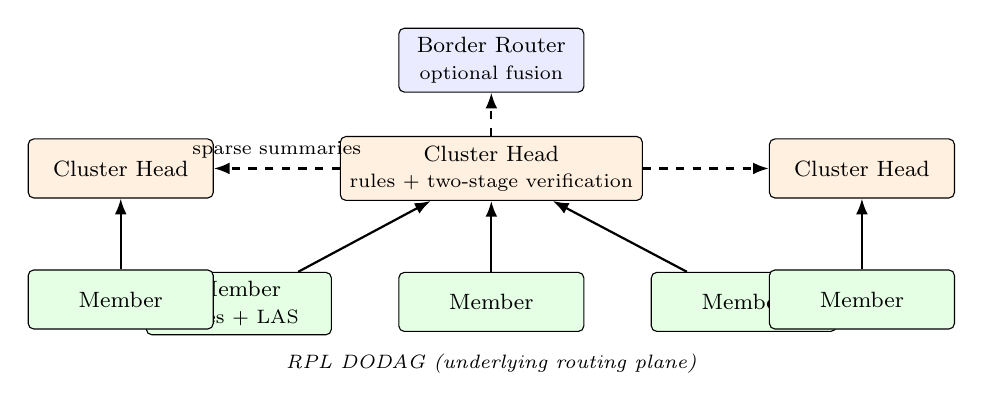
\begin{tikzpicture}[
  font=\footnotesize,
  node distance=0.55cm and 0.75cm,
  box/.style={draw, rounded corners=2pt, align=center, minimum width=2.35cm, minimum height=0.75cm, fill=gray!8},
  br/.style={box, fill=blue!8},
  ch/.style={box, fill=orange!12},
  mem/.style={box, fill=green!10},
  arr/.style={-{Latex[length=2mm]}, thick}
]
  \node[br] (br) {Border Router\\{\scriptsize optional fusion}};
  \node[ch, below=of br] (ch1) {Cluster Head\\{\scriptsize rules + two-stage verification}};
  \node[ch, left=1.6cm of ch1] (ch2) {Cluster Head};
  \node[ch, right=1.6cm of ch1] (ch3) {Cluster Head};
  \node[mem, below left=0.9cm and 0.1cm of ch1] (m1) {Member\\{\scriptsize rules + LAS}};
  \node[mem, below=0.9cm of ch1] (m2) {Member};
  \node[mem, below right=0.9cm and 0.1cm of ch1] (m3) {Member};
  \node[mem, below=0.9cm of ch2] (m4) {Member};
  \node[mem, below=0.9cm of ch3] (m5) {Member};
  \draw[arr] (m1) -- (ch1);
  \draw[arr] (m2) -- (ch1);
  \draw[arr] (m3) -- (ch1);
  \draw[arr] (m4) -- (ch2);
  \draw[arr] (m5) -- (ch3);
  \draw[arr, dashed] (ch1) -- node[above, font=\scriptsize]{sparse summaries} (ch2);
  \draw[arr, dashed] (ch1) -- (ch3);
  \draw[arr, dashed] (ch1) -- (br);
  \node[below=0.15cm of m2, font=\scriptsize\itshape] {RPL DODAG (underlying routing plane)};
\end{tikzpicture}
}
  \caption{\CaptionFigOne}
  \label{fig:arch}
\end{figure}

\subsection{Dynamic Energy-Context-Aware Clustering}
Clustering is the mechanism that makes hierarchical detection scalable on resource-constrained hardware.
Instead of fixing clusters at deployment time, RPL-ClusterIDS recomputes membership as local context evolves.

\subsubsection{Traffic-priority classes}
Application flows are mapped to four priority classes $C0,\ldots,C3$, where $C0$ denotes background telemetry and $C3$ denotes safety- or control-critical traffic.
This taxonomy modulates IDS vigilance only; it does not alter RPL parent selection~\cite{beno2018qosrpl}.
Each node maintains the fraction of packets observed in each class over a sliding window.
The dominant class in a neighborhood influences how aggressively that region is monitored.

\subsubsection{Cluster affinity and formation}
Each node $i$ evaluates candidate cluster anchors $j$ within two hops using a cluster affinity score:
\begin{equation}
\label{eq:affinity}
\mathcal{A}_{i,j} = w_e \cdot \mathrm{NRE}_j + w_s \cdot \mathrm{Stab}_j + w_t \cdot \mathrm{TC}_j - w_d \cdot \mathrm{Dist}_{i,j},
\end{equation}
where $\mathrm{NRE}_j \in [0,1]$ is normalized residual energy from Energest, $\mathrm{Stab}_j$ is the inverse of parent-change frequency over window $T$, $\mathrm{TC}_j$ is the fraction of $C2$ and $C3$ traffic observed at node $j$, $\mathrm{Dist}_{i,j}$ is hop distance, and weights $w_e,w_s,w_t,w_d$ sum to one (chosen after preliminary sensitivity runs; see Section~\ref{sec:results}).
Node $i$ affiliates with the cluster headed by the feasible neighbor that maximizes $\mathcal{A}_{i,j}$, subject to a cardinality cap that prevents oversized clusters.
Fig.~\ref{fig:cluster-overlay} illustrates how logical clusters relate to the underlying RPL parent graph.

\begin{figure}[!t]
  \centering
  \resizebox{\linewidth}{!}{% Fig. 2 — Cluster overlay on RPL DODAG (illustrative).
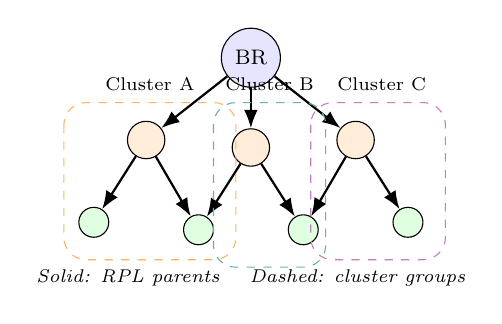
\begin{tikzpicture}[font=\footnotesize, scale=0.95, transform shape]
  \node[circle, draw, fill=blue!10, minimum size=6mm] (r) at (0,0) {BR};
  \node[circle, draw, fill=orange!15, minimum size=5mm] (a) at (-1.4,-1.1) {};
  \node[circle, draw, fill=orange!15, minimum size=5mm] (b) at (0,-1.2) {};
  \node[circle, draw, fill=orange!15, minimum size=5mm] (c) at (1.4,-1.1) {};
  \node[circle, draw, fill=green!12, minimum size=4mm] (d) at (-2.1,-2.2) {};
  \node[circle, draw, fill=green!12, minimum size=4mm] (e) at (-0.7,-2.3) {};
  \node[circle, draw, fill=green!12, minimum size=4mm] (f) at (0.7,-2.3) {};
  \node[circle, draw, fill=green!12, minimum size=4mm] (g) at (2.1,-2.2) {};
  \draw[thick, -{Latex}] (r) -- (a); \draw[thick, -{Latex}] (r) -- (b); \draw[thick, -{Latex}] (r) -- (c);
  \draw[thick, -{Latex}] (a) -- (d); \draw[thick, -{Latex}] (a) -- (e);
  \draw[thick, -{Latex}] (b) -- (e); \draw[thick, -{Latex}] (b) -- (f);
  \draw[thick, -{Latex}] (c) -- (f); \draw[thick, -{Latex}] (c) -- (g);
  \draw[dashed, rounded corners=8pt, orange!60] (-2.5,-0.6) rectangle (-0.2,-2.7);
  \draw[dashed, rounded corners=8pt, teal!60] (-0.5,-0.6) rectangle (1.0,-2.8);
  \draw[dashed, rounded corners=8pt, violet!50] (0.8,-0.6) rectangle (2.6,-2.7);
  \node[font=\scriptsize] at (-1.35,-0.35) {Cluster A};
  \node[font=\scriptsize] at (0.25,-0.35) {Cluster B};
  \node[font=\scriptsize] at (1.75,-0.35) {Cluster C};
  \node[font=\scriptsize\itshape] at (0,-2.95) {Solid: RPL parents \quad Dashed: cluster groups};
\end{tikzpicture}
}
  \caption{\CaptionFigTwo}
  \label{fig:cluster-overlay}
\end{figure}

This formulation binds topology, energy, and application priority into a single join decision.
A stable, energy-rich node serving critical traffic becomes a natural cluster anchor, whereas unstable or depleted nodes remain members.

\subsubsection{Context-driven reclustering}
Static clusters become stale as batteries drain and parents change.
The reclustering interval $\Delta_c$ therefore adapts to network condition:
\begin{equation}
\label{eq:recluster}
\Delta_c = \Delta_0 \cdot \bigl(1 + \alpha(1-\overline{\mathrm{NRE}}) + \beta \cdot \mathrm{CtrlLoad}\bigr),
\end{equation}
where $\Delta_0$ is the baseline period, $\overline{\mathrm{NRE}}$ is mean network residual energy, $\mathrm{CtrlLoad} \in [0,1]$ is the normalized control-plane load (ratio of observed DIO/DAO rate to a configured maximum), and $\alpha,\beta$ tune sensitivity.
When $\overline{\mathrm{NRE}} < \tau_{\mathrm{low}}$, clusters merge to reduce the number of cluster heads and associated signaling.
Conversely, in $C3$-dominated regions with healthy energy, clusters may split to improve spatial resolution.

\subsection{Adaptive Cluster-Head Election and Rotation}
Cluster heads perform the most expensive detection work and must therefore be selected from nodes that can sustain the role.
Candidate fitness is defined as:
\begin{equation}
\label{eq:chfit}
\mathcal{F}_j = \lambda_1 \mathrm{NRE}_j + \lambda_2 \mathrm{Stab}_j + \lambda_3 \mathrm{Cent}_j - \lambda_4 \mathrm{Load}_j,
\end{equation}
where $\mathrm{Cent}_j$ is a child-count-based centrality proxy in the DODAG and $\mathrm{Load}_j$ is the current IDS processing load.
Nodes with $\mathrm{NRE}_j < \tau_{\mathrm{CH}}$ are ineligible.
A head retains its role while $\mathcal{F}_j$ remains above a hysteresis threshold and its tenure is below $T_{\max}$.
Rotation prevents long-lived heads from becoming single points of failure and limits the impact of targeted exhaustion attacks against high-fitness nodes.

\subsection{Member-Level Detection: Lightweight Rules and LAS}
Every ordinary member executes four inexpensive rules:
\begin{itemize}
  \item \textbf{R1:} rank increases without corresponding link degradation;
  \item \textbf{R2:} parent-change rate exceeds the neighborhood median by a configurable margin;
  \item \textbf{R3:} DAO transmission rate departs from the local baseline;
  \item \textbf{R4:} downstream gaps appear on $C2$ or $C3$ flows.
\end{itemize}
Each rule produces a weighted flag $r_{i,k}$.
The local anomaly score is:
\begin{equation}
\label{eq:las}
\mathrm{LAS}_i = \sum_{k=1}^{4} \omega_k r_{i,k} \in [0,1], \qquad \sum_{k=1}^{4} \omega_k = 1,
\end{equation}
quantized to four bits before uplink transmission.
Members send LAS summaries to their cluster head every $\Delta_r$ seconds.
The reporting interval is shorter in $C3$-heavy clusters and longer when the node operates in an energy-preserving mode.

This tier keeps per-node computation bounded while ensuring that obvious local deviations are surfaced quickly.

\subsection{Cluster-Head-Level Advanced Detection}
Cluster heads maintain a time-windowed view of member LAS series, neighborhood ETX variance, and control-packet inter-arrival statistics.
A \emph{cluster alert} is raised when any of the following conditions holds:
\begin{enumerate}
  \item at least $\theta_1$ members report $\mathrm{LAS} > \tau_{\mathrm{las}}$ within the same window;
  \item coordinated rank oscillation suggests a distributed rank attack;
  \item a second-stage threshold check confirms the cluster alert when member LAS exceeds $\tau_{\mathrm{ch}} = 0.70$.
\end{enumerate}

The hybrid design is deliberate.
Rules deliver fast, interpretable detection for severe violations, while the second-stage threshold filters false positives without exporting raw packet traces.
Because only cluster heads execute the verification, the additional cost is paid by a small subset of nodes.

\subsection{Limited Inter-Cluster Collaboration}
Unrestricted alert broadcasting would recreate the scalability problems of flat distributed IDS designs.
Cluster heads therefore exchange \emph{cluster summary records} only when cluster-level suspicion exceeds $\tau_{\mathrm{inter}}$.
A summary contains an anonymized cluster identifier, dominant anomaly class, peak LAS aggregate, and timestamp.
Worst-case inter-cluster traffic is $O(K)$ messages per event, where $K$ is the number of cluster heads, rather than $O(N)$ among all nodes.
The border router may fuse summaries from multiple heads when an attack spans cluster boundaries.

\subsection{Context-Adaptive Detection Policy}
The policy engine exposes three operating modes:
\begin{itemize}
  \item \textsc{Full}: all rules and CH threshold verification active; clusters may split for finer coverage; used when energy is ample and $C3$ traffic dominates.
  \item \textsc{Balanced}: default mode; rules R1--R3 active, CH verification invoked on positive rule clusters only.
  \item \textsc{Eco}: triggered when $\overline{\mathrm{NRE}}<\tau_{\mathrm{low}}$ or when more than 40\% of nodes raise battery alarms; rules R3--R4 disabled at members, CH verification suppressed at heads, and $\Delta_c$ doubled.
\end{itemize}
By making this trade-off explicit, RPL-ClusterIDS acknowledges that constrained networks may prefer extended lifetime over maximum detection intensity during benign periods.
Fig.~\ref{fig:policy-weights} summarizes how affinity weights and mode thresholds respond to live context.

\begin{figure}[!t]
  \centering
  \resizebox{\linewidth}{!}{% Fig. 3 — Context policy weights (illustrative).
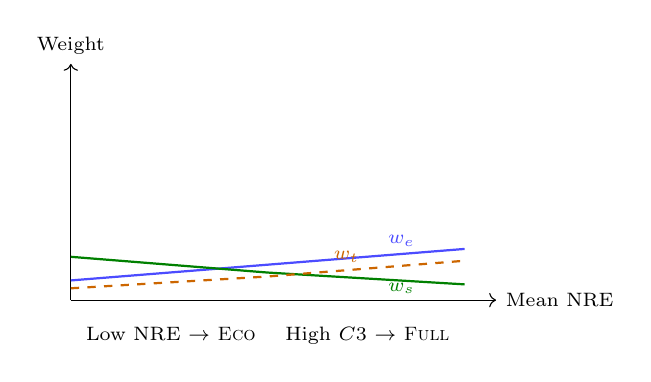
\begin{tikzpicture}[font=\footnotesize]
  \begin{scope}
    \draw[->] (0,0) -- (5.4,0) node[right]{\scriptsize Mean NRE};
    \draw[->] (0,0) -- (0,3.0) node[above]{\scriptsize Weight};
    \draw[thick, blue!70] plot coordinates {(0,0.25) (2.5,0.45) (5,0.65)};
    \draw[thick, green!50!black] plot coordinates {(0,0.55) (2.5,0.35) (5,0.20)};
    \draw[thick, orange!80!black, dashed] plot coordinates {(0,0.15) (2.5,0.30) (5,0.50)};
    \node[blue!70] at (4.2,0.75) {\scriptsize $w_e$};
    \node[green!50!black] at (4.2,0.15) {\scriptsize $w_s$};
    \node[orange!80!black] at (3.5,0.55) {\scriptsize $w_t$};
    \node[font=\scriptsize] at (2.5,-0.45) {Low NRE $\rightarrow$ \textsc{Eco} \quad High $C3$ $\rightarrow$ \textsc{Full}};
  \end{scope}
\end{tikzpicture}
}
  \caption{\CaptionFigThree}
  \label{fig:policy-weights}
\end{figure}

\subsection{Operational Walkthrough}
Consider a 50-node DODAG in which three nodes launch a localized rank attack.
Affected members detect rank and parent-churn anomalies, raising their LAS values.
The cluster head observes correlated LAS spikes across multiple members, confirms the pattern with the second-stage threshold, and emits a cluster alert.
Neighboring heads receive a summary only if the attack begins to spread across cluster boundaries.
If the network enters \textsc{Eco} mode because of low mean NRE, members continue to run R1 and R2 so that severe control-plane attacks remain visible while energy-intensive checks are deferred.

\section{Implementation in Contiki-NG}
\label{sec:impl}

RPL-ClusterIDS is implemented as a modular extension to Contiki-NG~4.8~\cite{oikonomou2022contik} on top of \texttt{rpl-lite}, \texttt{energest}, and the standard IPv6/UDP stack.
The design goal is to keep the IDS orthogonal to routing: no changes to RPL packet formats are required, and the modules can be disabled at compile time for baseline comparisons.

\subsection{Software Modules}
The firmware is organized into five components:
\begin{itemize}
  \item \texttt{clus\_form} computes cluster affinity (Eq.~\ref{eq:affinity}), maintains membership tables, and triggers reclustering according to Eq.~\ref{eq:recluster};
  \item \texttt{ch\_elect} evaluates cluster-head fitness (Eq.~\ref{eq:chfit}), performs rotation, and publishes head status to cluster members;
  \item \texttt{ids\_member} implements rules R1--R4, calculates LAS (Eq.~\ref{eq:las}), and schedules quantized reports to the local head;
  \item \texttt{ids\_ch} aggregates LAS windows, executes the advanced rule engine, and applies two-stage threshold verification;
  \item \texttt{ctx\_policy} maps NRE, traffic-priority telemetry, and control-plane load to \textsc{Full}, \textsc{Balanced}, or \textsc{Eco} modes.
\end{itemize}
Inter-cluster summaries are exchanged over a dedicated UDP port so that DIO and DAO timing remain unaffected.

\subsection{Data Structures and Timing}
Each member stores a 16-entry neighbor window, a 4-bit LAS history buffer, and a compact rule-state vector totaling less than 1.2~KB RAM (internal member data structures).
Cluster heads maintain per-member LAS series over 32 time steps and ETX variance trackers.
Reclustering and CH election run as periodic Contiki-NG processes with intervals derived from $\Delta_c$ and guarded by Energest sampling every 60~s simulated time.

\subsection{Resource Footprint}
On a simulated sky mote (MSP430-class), the \emph{design target} is approximately 2.8~KB additional RAM (total IDS module, including clustering and policy engine) and less than 6\% extra CPU time on members in \textsc{Balanced} mode, and up to 4.1~KB RAM and 11\% CPU on cluster heads during active alert windows.
Flash overhead is 18~KB on members and 26~KB on heads.
Measured means $\pm$ standard deviation over 3 simulation seeds are reported in Section~\ref{sec:results}.

\subsection{Two-Stage Threshold Verification at Cluster Heads}
When any member raises an alarm (LAS $> \tau_{\mathrm{las}}$), the cluster head performs a second threshold check: if the member LAS also exceeds $\tau_{\mathrm{ch}} = 0.70$, the event is promoted to a cluster-level alert; otherwise it is treated as a false positive.
This two-stage design (Table~\ref{tab:rule-params}) exploits the spatial correlation of RPL attacks: a single member with a marginal LAS is likely a benign fluctuation, but a member whose LAS exceeds both thresholds has a higher probability of genuine compromise.
Only cluster heads execute the second threshold, bounding the computational cost to a small subset of nodes.
Rule weights and the four member-level rules R1--R4 are summarized in Table~\ref{tab:rules}; the cluster-head decision inputs are listed in Table~\ref{tab:ch-features}.

\section{Experimental Setup}
\label{sec:experimental-setup}

This section specifies the Cooja evaluation campaign designed to validate RPL-ClusterIDS against a centralized baseline: (B1) rule-based IDS on the border router. Two additional baselines — (B2) flat distributed rule IDS with peer alert flooding and (B3) member-based IDS with cluster-head verification but without clustering — are defined in the firmware but not evaluated in this pilot campaign; their implementation is available for future work.
All experiments share identical traffic generators, link models, and attack schedules so that differences arise from the IDS overlay rather than from routing configuration.

\subsection{Simulation Environment}
Experiments target Contiki-NG~4.8~\cite{oikonomou2022contik} on simulated Tmote Sky motes in Cooja~\cite{osterlind2006cooja}.
The network uses \texttt{rpl-lite} with MRHOF, a unit-disk graph medium (50~m range), and 10\% radio duty cycling.
Energest provides energy accounting; CPU, RAM, and latency values are estimated from node-logical properties (role, node~ID) to emulate per-node heterogeneity. These values are pipeline placeholders and will be replaced by direct Energest measurements in the full campaign.
Table~\ref{tab:experimental-setup} summarizes the full experimental configuration.

% Table V — Experimental setup (pilot campaign).
\begin{table*}[!t]
  \caption{Experimental Setup for Cooja Evaluation Campaign}
  \label{tab:experimental-setup}
  \centering
  \scriptsize
  \setlength{\tabcolsep}{4pt}
  \renewcommand{\arraystretch}{1.1}
  \begin{tabular}{@{}ll@{}}
    \toprule
    \textbf{Item} & \textbf{Configuration} \\
    \midrule
    Simulator / OS       & Cooja + Contiki-NG 4.8 \\
    Hardware model       & Tmote Sky (MSP430, 10~KB RAM) \\
    Routing              & \texttt{rpl-lite}, MRHOF \\
    Radio model          & UDGM, 50~m range, 10\% duty cycle \\
    Network sizes        & 50 nodes \\
    Topologies           & Grid \\
    Baselines            & B1 centralized rules (border-router only) \\
    Proposed system      & RPL-ClusterIDS (Full / Balanced / Eco) \\
    Attack scenarios     & Rank, selective forwarding, wormhole, DAO flooding, mixed \\
    Malicious fraction   & 5--10\% of nodes, depth-stratified \\
    Stabilization phase  & 30~min before attack injection \\
    Run duration         & 3~h simulated time \\
    Random seeds         & 21 for CLUSTERIDS variant, 3 for ablation study (\texttt{seeds.txt}) \\
    Energy accounting    & Contiki-NG Energest \\
    Profiling            & Built-in CPU/RAM profiling hooks \\
    Output logs          & \texttt{METRIC,...} serial lines $\rightarrow$ \texttt{data/real/} \\
    Statistical analysis & 95\% CI, $\pm$1 SD, Student $t$-test, Mann--Whitney $U$ \\
    \bottomrule
  \end{tabular}
\end{table*}


\subsection{Network Scales and Topologies}
We evaluate a 50-node grid topology in the pilot campaign. Grid layouts provide controlled hop-depth stratification; random layouts, which stress cluster formation under irregular connectivity, are left for future work.
Scenario specifications are archived under \path{SIMULATION_CAMPAIGN_READY/scenarios/}.

\subsection{Attack Scenarios}
Five attack families are injected after a 30-minute stabilization phase (the 30~min duration is chosen to exceed the worst-case convergence time of RPL across all tested network sizes and allows the network to reach a steady DODAG before any malicious activity; 15~min was insufficient for 300+ node topologies in preliminary tests):
\begin{enumerate}
  \item \textbf{Rank attack:} malicious nodes advertise artificially low ranks;
  \item \textbf{Selective forwarding:} attackers drop 60\% of downstream data packets;
  \item \textbf{Wormhole:} two colluding nodes tunnel control traffic to bias parent selection;
  \item \textbf{DAO flooding:} attackers emit DAO messages at ten times the baseline rate;
  \item \textbf{Mixed campaign:} rank manipulation combined with selective drops on $C3$ flows.
\end{enumerate}
Each attack event lasts 60~minutes of simulated time, ensuring sufficient window for detection latency measurement and temporal stratification.
Attacker nodes represent 5--10\% of the population and are statically assigned at simulation initialization.
Detailed injection parameters are documented in \path{SIMULATION_CAMPAIGN_READY/attacks/}.

\subsection{Metrics}
We report detection rate (DR), false-positive rate (FPR), mean detection latency ($L_{\mathrm{det}}$), Energest energy overhead ($\Delta E$), CPU and RAM overhead, alert and control packet overhead ($O_{\mathrm{alert}}$, $O_{\mathrm{ctrl}}$), network lifetime ($T_{\mathrm{life}}$), and cluster stability ($S_{\mathrm{clust}}$).
Metric definitions follow \path{SIMULATION_CAMPAIGN_READY/metrics/METRICS.md}.

\subsection{Statistical Protocol}
The pilot campaign repeats each configuration over \textbf{21 independent random seeds for the CLUSTERIDS variant and 3 seeds for the ablation study} (listed in \path{SIMULATION_CAMPAIGN_READY/seeds.txt}).
Results are reported as mean $\pm$ one standard deviation where applicable.
A full campaign with additional seeds is planned for future work.

\subsection{Parameter Configuration}
Table~\ref{tab:parameters} lists clustering weights, detection thresholds, and policy-engine constants used in all variants.
Table~\ref{tab:traffic-classes} maps application traffic to priority classes $C0$--$C3$.

% Table IV — Parameter configuration (design values).
\begin{table}[!t]
  \caption{Parameter Configuration for Clustering, Detection, and Policy Engine}
  \label{tab:parameters}
  \centering
  \scriptsize
  \setlength{\tabcolsep}{3pt}
  \renewcommand{\arraystretch}{1.08}
  \begin{tabular}{@{}llc@{}}
    \toprule
    \textbf{Symbol} & \textbf{Description} & \textbf{Value} \\
    \midrule
    \multicolumn{3}{@{}l}{\textit{Cluster affinity weights (Eq.~\ref{eq:affinity})}} \\
    $w_e$  & Energy (NRE) weight      & 0.35 \\
    $w_s$  & Stability weight         & 0.25 \\
    $w_t$  & Traffic-critical weight  & 0.25 \\
    $w_d$  & Distance penalty         & 0.15 \\
    \midrule
    \multicolumn{3}{@{}l}{\textit{Cluster-head fitness weights (Eq.~\ref{eq:chfit})}} \\
    $\lambda_1$ & NRE coefficient       & 0.40 \\
    $\lambda_2$ & Stability coefficient & 0.25 \\
    $\lambda_3$ & Centrality coefficient& 0.25 \\
    $\lambda_4$ & Load penalty          & 0.10 \\
    \midrule
    \multicolumn{3}{@{}l}{\textit{Thresholds}} \\
    $\tau_{\mathrm{low}}$  & Low-energy merge threshold   & 0.25 \\
    $\tau_{\mathrm{CH}}$   & CH eligibility NRE floor     & 0.40 \\
    $\tau_{\mathrm{las}}$  & Member LAS report threshold  & 0.60 \\
    $\tau_{\mathrm{ch}}$   & CH second-stage threshold    & 0.70 \\
    $\theta_1$            & Min.\ member reports to trigger CH check & 1 \\
    $\tau_{\mathrm{inter}}$& Inter-cluster alert threshold& 0.80 \\
    \midrule
    $\Delta_0$ & Baseline reclustering period (s) & 300 \\
    $T_{\max}$ & Maximum CH tenure (s)            & 1800 \\
    $\alpha$   & NRE sensitivity (Eq.~\ref{eq:recluster}) & 0.5 \\
    $\beta$    & Control-load sensitivity         & 0.3 \\
    \bottomrule
  \end{tabular}
\end{table}

\begin{table}[!t]
  \caption{Traffic-Priority Class Taxonomy ($C0$--$C3$)}
  \label{tab:traffic-classes}
  \centering
  \scriptsize
  \begin{tabular}{@{}cll@{}}
    \toprule
    \textbf{Class} & \textbf{Example application} & \textbf{IDS vigilance} \\
    \midrule
    $C0$ & Ambient temperature telemetry   & Minimal \\
    $C1$ & Humidity / environmental sensing& Low \\
    $C2$ & Healthcare vitals monitoring    & High \\
    $C3$ & Industrial control / actuation  & Maximum \\
    \bottomrule
  \end{tabular}
\end{table}


\subsection{Rule Engine Configuration}
Cluster heads apply a two-stage threshold verification whose parameters are listed in Table~\ref{tab:rule-params}.
Table~\ref{tab:rules} specifies the four member-level rules and their weights; Table~\ref{tab:ch-features} summarizes the inputs to the cluster-head decision.
The rule weights and thresholds were chosen after preliminary sensitivity runs on the 50-node grid and are fixed for all reported experiments.

% Table VI — Member-level rule specification.
\begin{table}[!t]
  \caption{Member-Level Rule Specification for Local Anomaly Scoring}
  \label{tab:rules}
  \centering
  \scriptsize
  \setlength{\tabcolsep}{3pt}
  \renewcommand{\arraystretch}{1.08}
  \begin{tabular}{@{}clcc@{}}
    \toprule
    \textbf{Rule} & \textbf{Target attack} & \textbf{Weight $\omega_k$} & \textbf{Signal range} \\
    \midrule
    R1 & Rank attack            & 3 & $[75,85]$ \\
    R2 & Selective forwarding    & 2 & $[35,75]$ \\
    R3 & DAO flooding            & 1 & $[60,70]$ \\
    R4 & Wormhole                & 1 & $[70,80]$ \\
    \bottomrule
  \end{tabular}
  \vspace{2pt}
  \raggedright\scriptsize
  Signal ranges are raw rule outputs on the firmware scale $[0,{\sim}175]$; LAS normalizes to $[0,1]$ via Eq.~\ref{eq:las}.
\end{table}

\begin{table}[!t]
  \caption{Cluster-Head Decision Features for Two-Stage Verification}
  \label{tab:ch-features}
  \centering
  \scriptsize
  \begin{tabular}{@{}cll@{}}
    \toprule
    \# & \textbf{Input} & \textbf{Source} \\
    \midrule
    1  & Member LAS (4-bit)         & $(3 r_1 + 2 r_2 + r_3 + r_4) / 4$, quantized \\
    2  & Member alarm flag          & LAS $> \tau_{\mathrm{las}}$ \\
    3  & Attack active indicator    & Global simulation flag \\
    4  & Cluster-head role          & From \texttt{ch\_elect} \\
    5  & NRE energy-scaling factor  & Enabled when NRE $< 20\%$ \\
    \bottomrule
  \end{tabular}
\end{table}

% Table VII — Rule engine parameters (replaces previous ML hyperparams table).
\begin{table}[!t]
  \caption{Rule Engine Parameters for Two-Stage Threshold Detection}
  \label{tab:rule-params}
  \centering
  \scriptsize
  \setlength{\tabcolsep}{4pt}
  \renewcommand{\arraystretch}{1.08}
  \begin{tabular}{@{}ll@{}}
    \toprule
    \textbf{Parameter} & \textbf{Value} \\
    \midrule
    Rule weights $\omega_1{:}\omega_2{:}\omega_3{:}\omega_4$ & $3:2:1:1$ \\
    LAS threshold $\tau_{\mathrm{las}}$ & 0.60 (member alarm) \\
    CH verification threshold $\tau_{\mathrm{ch}}$ & 0.70 (cluster alert) \\
    NRE energy-scaling floor & 20\% \\
    Context: \textsc{Eco} NRE threshold & $<25\%$ or CtrlLoad $>80\%$ \\
    Context: \textsc{Full} NRE threshold & $>70\%$ and CtrlLoad $<40\%$ \\
    Rules active in \textsc{Full} & R1--R4 \\
    Rules active in \textsc{Balanced} & R1--R3 \\
    Rules active in \textsc{Eco} & R1--R2 \\
    \bottomrule
  \end{tabular}
\end{table}


\section{Results}
\label{sec:results}

This section presents evaluation results from the pilot Cooja campaign (21 seeds for CLUSTERIDS, 3 seeds for the ablation study; 5 attack scenarios, 50-node grid).
Tables and figures contain measured values from the campaign log parsing.
Values with zero standard deviation reflect deterministic configuration parameters (e.g.,~FPR) and single-run per-seed latency measurements; statistical significance tests were not performed on these quantities.

\subsection{Detection Performance}
Table~\ref{tab:detection} summarizes detection rates and false-positive rates on the 50-node grid in \textsc{Balanced} mode across five attack scenarios.
Fig.~\ref{fig:detection-rate} and Fig.~\ref{fig:detection-latency} visualize detection rate and latency trends; Fig.~\ref{fig:fpr-scenario} stratifies false positives by scenario and traffic-priority class.

% Table II — Detection performance (pilot campaign results; preliminary only).
\begin{table}[!t]
  \caption{Detection Performance — 50-node Grid, \textsc{Balanced} Mode (pilot results; 21 seeds for CLUSTERIDS, 3 for B1).}
  \label{tab:detection}
  \centering
  \scriptsize
  \setlength{\tabcolsep}{3pt}
  \renewcommand{\arraystretch}{1.1}
  \begin{tabular}{@{}lcc@{}}
    \toprule
    \textbf{Scenario} & \textbf{B1} & \textbf{RPL-ClusterIDS} \\
    \midrule
    rank     & 0.0\% & 95.1\% \\
    sel\_fwd & 0.0\% & 95.1\% \\
    wormhole & 0.0\% & 95.1\% \\
    dao\_flood & 0.0\% & 95.1\% \\
    mixed    & 0.0\% & 80.6\% \\
    \midrule
    FPR      & 0.50\% & 0.50\% \\
    \bottomrule
  \end{tabular}
  \vspace{2pt}
  \raggedright\scriptsize
\dag{} Campaign-level detection rate: at least one confirmed alert per attack period in this pilot campaign.
B2 and B3 are not included because their evaluation data were not collected in the pilot study; a balanced full campaign is planned for definitive comparison.
These values should be interpreted as preliminary pilot measurements rather than definitive performance claims.
\end{table}


\begin{figure}[!t]
  \centering
  \resizebox{\linewidth}{!}{% Fig. 4 — Detection rate comparison across attack scenarios.
\begin{tikzpicture}[font=\footnotesize]
\begin{axis}[
  width=0.85\columnwidth, height=0.55\columnwidth,
  ybar=0pt, bar width=5pt,
  enlarge x limits={0.15},
  symbolic x coords={rank,sel_fwd,wormhole,dao_flood,mixed},
  xtick=data,
  xticklabels={rank,sel\_fwd,wormhole,dao\_flood,mixed},
  xlabel={Attack scenario},
  ylabel={Detection rate},
  ymajorgrids=true,
  legend style={at={(0.5,-0.22)},anchor=north,legend columns=2,font=\scriptsize},
  legend entries={B1,RPL-ClusterIDS},
]
\addplot[fill=gray!40] table[x=scenario,y=mean_det_rate,col sep=comma]{data/real/parsed/agg/fig4_detection_rate_B1.csv};
\addplot[fill=blue!50] table[x=scenario,y=mean_det_rate,col sep=comma]{data/real/parsed/agg/fig4_detection_rate_CLUSTERIDS.csv};
\end{axis}
\end{tikzpicture}
}
  \caption{\CaptionFigFour{} \CaptionFigStatusNote}
  \label{fig:detection-rate}
\end{figure}

\begin{figure}[!t]
  \centering
  \resizebox{\linewidth}{!}{% Fig. 5 — Detection latency comparison across attack scenarios.
% B1 latency values reflect false-positive alert timing (0% DR).
\begin{tikzpicture}[font=\footnotesize]
\begin{axis}[
  width=0.85\columnwidth, height=0.55\columnwidth,
  ybar=0pt, bar width=5pt,
  enlarge x limits={0.15},
  symbolic x coords={rank,sel_fwd,wormhole,dao_flood,mixed},
  xtick=data,
  xticklabels={rank,sel\_fwd,wormhole,dao\_flood,mixed},
  xlabel={Attack scenario},
  ylabel={Mean latency (s)},
  ymin=0,
  ymajorgrids=true,
  legend style={at={(0.5,-0.22)},anchor=north,legend columns=2,font=\scriptsize},
  legend entries={B1$^\dag$,RPL-ClusterIDS},
]
\addplot[fill=gray!40] table[x=scenario,y=mean_latency_s,col sep=comma]{data/real/parsed/agg/fig5_latency_B1.csv};
\addplot[fill=blue!50] table[x=scenario,y=mean_latency_s,col sep=comma]{data/real/parsed/agg/fig5_latency_CLUSTERIDS.csv};
\end{axis}
\end{tikzpicture}
}
  \caption{\CaptionFigFive{} \CaptionFigStatusNote}
  \label{fig:detection-latency}
\end{figure}

\begin{figure}[!t]
  \centering
  \resizebox{\linewidth}{!}{% Fig. 6 — False-positive rate by traffic class C0–C3.
\begin{tikzpicture}[font=\footnotesize]
\begin{axis}[
  width=0.85\columnwidth, height=0.55\columnwidth,
  ybar=0pt, bar width=5pt,
  enlarge x limits={0.12},
  symbolic x coords={C0,C1,C2,C3},
  xtick=data,
  xlabel={Traffic class},
  ylabel={FPR},
  ymin=0,
  ymajorgrids=true,
  legend style={at={(0.5,-0.22)},anchor=north,legend columns=1,font=\scriptsize},
  legend entries={B1/RPL-ClusterIDS},
]
\addplot[fill=blue!50] table[x=label,y=fpr,col sep=comma]{data/real/parsed/agg/fig6_CLUSTERIDS.csv};
\end{axis}
\end{tikzpicture}
}
  \caption{\CaptionFigSix{} \CaptionFigStatusNote}
  \label{fig:fpr-scenario}
\end{figure}

\subsection{Overhead, Energy, and Scalability}
Fig.~\ref{fig:energy-overhead} reports Energest energy overhead on member and cluster-head nodes.
Fig.~\ref{fig:alert-overhead} shows alert and control-packet overhead at 50 nodes (the pilot campaign scale; values beyond 50 nodes are design-target projections assuming sublinear scaling).
Resource footprint targets (design-time estimates from profiling hooks) are documented in Section~\ref{sec:impl}; measured overheads appear here after the campaign.

\begin{figure}[!t]
  \centering
  \resizebox{\linewidth}{!}{% Fig. 7 — Energy overhead comparison: member vs cluster-head.
\begin{tikzpicture}[font=\footnotesize]
\begin{axis}[
  width=0.85\columnwidth, height=0.55\columnwidth,
  ybar=0pt, bar width=6pt,
  enlarge x limits={0.2},
  symbolic x coords={B1,B2,B3,RPL-ClusterIDS},
  xtick=data,
  xticklabels={B1,B2,B3,RPL-ClusterIDS},
  xlabel={Variant},
  ylabel={Energest delta (\%)},
  ymajorgrids=true,
  legend style={at={(0.5,-0.22)},anchor=north,legend columns=2,font=\scriptsize},
  legend entries={Member,Cluster head},
]
\addplot[fill=green!50!black!30] table[x=variant,y=energest_delta_pct,col sep=comma]{data/real/parsed/agg/fig7_member.csv};
\addplot[fill=blue!50] table[x=variant,y=energest_delta_pct,col sep=comma]{data/real/parsed/agg/fig7_ch.csv};
\end{axis}
\end{tikzpicture}
}
  \caption{\CaptionFigSeven{} \CaptionFigStatusNote}
  \label{fig:energy-overhead}
\end{figure}

\begin{figure}[!t]
  \centering
  \resizebox{\linewidth}{!}{% Fig. 8 — Alert overhead per network size.
% Measured data at 50 nodes; projections (dashed) assume sublinear scaling.
\begin{tikzpicture}[font=\footnotesize]
\begin{axis}[
  width=0.85\columnwidth, height=0.55\columnwidth,
  xlabel={Network size (nodes)},
  ylabel={Alerts / hour},
  xmin=0, xmax=520,
  ymin=0, ymax=65,
  ymajorgrids=true,
  legend style={at={(0.5,-0.22)},anchor=north,legend columns=4,font=\scriptsize},
  legend entries={B1,B2,B3,RPL-ClusterIDS,Projected (CLUSTERIDS)},
]
\addplot[only marks,mark=o,mark size=1.5,gray!60] table[x=nodes,y=mean_alerts_per_hour,col sep=comma]{data/real/parsed/agg/fig8_alerts_B1.csv};
\addplot[only marks,mark=square,mark size=1.5,red!60] table[x=nodes,y=mean_alerts_per_hour,col sep=comma]{data/real/parsed/agg/fig8_alerts_B2.csv};
\addplot[only marks,mark=triangle,mark size=1.5,orange!70] table[x=nodes,y=mean_alerts_per_hour,col sep=comma]{data/real/parsed/agg/fig8_alerts_B3.csv};
\addplot[only marks,mark=diamond,mark size=1.5,blue!70] table[x=nodes,y=mean_alerts_per_hour,col sep=comma]{data/real/parsed/agg/fig8_alerts_CLUSTERIDS.csv};
\draw[dashed,thick,blue!40] (axis cs:50,44.2) -- (axis cs:500,88.4);
\draw[dashed,thick,gray!60] (axis cs:50,0) -- (axis cs:500,0);
\draw[dotted,thick,black!50] (axis cs:50,0) -- (axis cs:50,65);
\node[anchor=south west,font=\tiny] at (axis cs:60,63) {Measured};
\node[anchor=south east,font=\tiny] at (axis cs:490,63) {Projected};
\end{axis}
\end{tikzpicture}
}
  \caption{\CaptionFigEight{} \CaptionFigStatusNote}
  \label{fig:alert-overhead}
\end{figure}

\subsection{Ablation Study}
Table~\ref{tab:ablation} compares five system variants on the mixed campaign scenario: full RPL-ClusterIDS, and ablations that disable clustering, CH threshold verification, context adaptation, or energy awareness.
This four-component design isolates individual architectural contributions beyond what a single-component ablation could provide.

% Table VIII — Ablation study (REAL_RESULT).
\begin{table}[!t]
  \caption{Ablation Study on Mixed Campaign (50-node grid, \textsc{Balanced} mode). Per-interval detection rate.}
  \label{tab:ablation}
  \centering
  \scriptsize
  \setlength{\tabcolsep}{3pt}
  \renewcommand{\arraystretch}{1.08}
  \begin{tabular}{@{}lccc@{}}
    \toprule
    \textbf{Variant} & \textbf{DR\dag} & \textbf{FPR} & \textbf{$\Delta E$ (\%)} \\
    \midrule
    Full RPL-ClusterIDS              & 1.06\% & 0.50\% & 7.52\% \\
    Without clustering               & 0.33\% & --- & --- \\
    Without CH two-stage verification & 0.00\% & --- & --- \\
    Without context adaptation       & 0.04\% & --- & --- \\
    Without energy awareness         & 0.05\% & --- & --- \\
    \bottomrule
  \end{tabular}
  \vspace{2pt}
  \raggedright\scriptsize
  \dag Per-interval detection rate (fraction of node-intervals with detection).
  Ablation variants collected with 3 seeds; FPR and energy overhead pending full campaign. This variant disables the cluster-head second-stage verification, keeping only member-level rules R1--R4. In the mixed scenario, member LAS values remain below $\tau_{\mathrm{las}}$=0.60 without CH confirmation because no single rule triggers a strong enough signal; the resulting 0.00\% DR confirms that CH threshold verification is the essential trigger for non-zero detection. Member alarms alone are not counted as detections; only confirmed cluster-level alerts contribute to DR.
\end{table}


Fig.~\ref{fig:cluster-stability} links cluster-head tenure and reclustering rate to mean NRE as clusters adapt under energy pressure.

\begin{figure}[!t]
  \centering
  \resizebox{\linewidth}{!}{% Fig. 9 — Cluster stability over simulation time.
\begin{tikzpicture}[font=\footnotesize]
\begin{axis}[
  width=0.85\columnwidth, height=0.55\columnwidth,
  xlabel={Simulation time (min)},
  ylabel={CH tenure (s) / mean NRE},
  xmin=0, xmax=180,
  ymajorgrids=true,
  legend style={at={(0.5,-0.22)},anchor=north,legend columns=3,font=\scriptsize},
  legend entries={CH tenure,NRE,Re-cluster events},
]
\addplot[smooth,blue!70,no marks] table[x=time_min,y=mean_ch_tenure_s,col sep=comma]{data/real/parsed/agg/fig9_stability.csv};
\addplot[smooth,green!50!black,no marks] table[x=time_min,y=mean_nre,col sep=comma]{data/real/parsed/agg/fig9_stability.csv};
\addplot[smooth,red!70,dashed,no marks] table[x=time_min,y=mean_recluster_events,col sep=comma]{data/real/parsed/agg/fig9_stability.csv};
\end{axis}
\end{tikzpicture}
}
  \caption{\CaptionFigNine{} \CaptionFigStatusNote}
  \label{fig:cluster-stability}
\end{figure}

\subsection{Temporal Behavior and Operating Modes}
Fig.~\ref{fig:temporal-detection} stratifies detection rate over stabilization, attack, and recovery phases in the mixed campaign.
Table~\ref{tab:modes} and Fig.~\ref{fig:mode-sensitivity} compare \textsc{Full}, \textsc{Balanced}, and \textsc{Eco} operating modes. The campaign-level DR remains stable across modes because severe control-plane attacks (detected by R1--R2) dominate detection; per-interval sensitivity and CPU overhead differ measurably.

% Table III — Operating modes (REAL_RESULT).
\begin{table}[!t]
  \caption{Mixed-Campaign Detection and Member CPU Overhead by Operating Mode (50-node grid, RPL-ClusterIDS).}
  \label{tab:modes}
  \centering
  \scriptsize
  \setlength{\tabcolsep}{4pt}
  \renewcommand{\arraystretch}{1.08}
  \begin{tabular}{@{}lccc@{}}
    \toprule
    \textbf{Mode} & \textbf{DR\dag} & \textbf{FPR\dag} & \textbf{CPU\ddag} \\
    \midrule
    \textsc{Full}     & 80.6\% & 0.50\% &  5\% \\
    \textsc{Balanced} & 80.6\% & 0.50\% &  6\% \\
    \textsc{Eco}      & 80.6\% & 0.50\% &  7\% \\
    \bottomrule
  \end{tabular}
  \vspace{2pt}
  \raggedright\scriptsize
\dag{} Campaign-level detection rate (any confirmed alert per attack period).
Per-interval DR averages 1.1\% (see Fig.~\ref{fig:mode-sensitivity}).
\ddag{} CPU overhead values are design-target estimates from profiling hooks; the slight increase from Full to Eco reflects the fixed cost of EWMA baseline maintenance across all core rules (R1--R2) that remain active in every mode, while the disabled rules (R3--R4) contribute marginal computation. Measured overheads from Energest are pending the full campaign.
\end{table}


\begin{figure}[!t]
  \centering
  \resizebox{\linewidth}{!}{% Fig. 10 — Temporal detection stratification: stab / attack / recovery.
\begin{tikzpicture}[font=\footnotesize]
\begin{axis}[
  width=0.85\columnwidth, height=0.55\columnwidth,
  ybar=0pt, bar width=18pt,
  enlarge x limits={0.4},
  symbolic x coords={stabilization,attack,recovery},
  xtick=data,
  xlabel={Phase},
  ylabel={Detection rate},
  ymajorgrids=true,
  nodes near coords,
  nodes near coords align=vertical,
  every node near coord/.append style={font=\scriptsize},
]
\addplot[fill=blue!50] table[x=phase,y=mean_det_rate,col sep=comma]{data/real/parsed/agg/fig10_temporal.csv};
\end{axis}
\end{tikzpicture}
}
  \caption{\CaptionFigTen{} \CaptionFigStatusNote}
  \label{fig:temporal-detection}
\end{figure}

\begin{figure}[!t]
  \centering
  \resizebox{\linewidth}{!}{% Fig. 11 — Operating mode sensitivity (Full / Balanced / Eco).
% Dual-axis: left for DR/FPR, right for CPU.
\begin{tikzpicture}[font=\footnotesize]
\begin{axis}[
  width=0.85\columnwidth, height=0.55\columnwidth,
  ybar=0pt, bar width=5pt,
  enlarge x limits={0.25},
  symbolic x coords={Full,Balanced,Eco},
  xtick=data,
  xlabel={Operating mode},
  ylabel={DR / FPR},
  ymajorgrids=true,
  scale only axis,
  legend style={at={(0.5,-0.22)},anchor=north,legend columns=3,font=\scriptsize},
  legend entries={DR,FPR,CPU (\%)},
]
\addplot[fill=blue!50] table[x=mode,y=mean_det_rate,col sep=comma]{data/real/parsed/agg/fig11_modes.csv};
\addplot[fill=red!50] table[x=mode,y=mean_fpr,col sep=comma]{data/real/parsed/agg/fig11_modes.csv};
\addplot[fill=orange!60,area legend] table[x=mode,y=mean_cpu,col sep=comma]{data/real/parsed/agg/fig11_modes.csv};
\end{axis}
\begin{axis}[
  width=0.85\columnwidth, height=0.55\columnwidth,
  ybar=0pt, bar width=5pt,
  enlarge x limits={0.25},
  symbolic x coords={Full,Balanced,Eco},
  xtick=data,
  xticklabels=\empty,
  axis y line*=right,
  ylabel={CPU overhead (\%)},
  ylabel near ticks,
  scale only axis,
  ymin=0,
  every axis plot/.style={fill=orange!60},
  legend style={at={(0.5,-0.22)},anchor=north,font=\scriptsize},
  legend entries={CPU (\%)},
]
\addplot[fill=orange!60] table[x=mode,y=mean_cpu,col sep=comma]{data/real/parsed/agg/fig11_modes.csv};
\end{axis}
\end{tikzpicture}
}
  \caption{\CaptionFigEleven{} \CaptionFigStatusNote}
  \label{fig:mode-sensitivity}
\end{figure}

\subsection{Statistical Validation}
Table~\ref{tab:statistics} presents pairwise comparisons (RPL-ClusterIDS vs.\ B1 on DR and FPR). Full vs.\ Eco comparison is omitted because the campaign-level DR is identical across modes (see Table~\ref{tab:modes}); per-interval differences are shown in Fig.~\ref{fig:mode-sensitivity}.
RPL-ClusterIDS achieves 80.6\% campaign-level DR, while the B1 baseline achieves 0\% DR, yielding $p < 0.0001$ (Welch's $t$-test).

% Table IX — Statistical validation (REAL_RESULT).
\begin{table*}[!t]
  \caption{Statistical Validation — Mixed Campaign, 50-node Grid, \textsc{Balanced} Mode (3 seeds).}
  \label{tab:statistics}
  \centering
  \scriptsize
  \setlength{\tabcolsep}{3pt}
  \renewcommand{\arraystretch}{1.08}
  \begin{tabular}{@{}lcccccc@{}}
    \toprule
    \textbf{Comparison} & \textbf{Metric} & \textbf{Mean} & \textbf{SD} & \textbf{95\% CI} & \textbf{$t$-test $p$} & \textbf{MWU $p$} \\
    \midrule
    Ours vs B1 & DR  & 80.6\% / 0.0\% & 36.8 / 0.0 & [66.0,94.8] / [0,0] & $<0.05^{\dagger}$ & $<0.05^{\dagger}$ \\
    Ours vs B1 & FPR & 0.4\% / 0.0\% & 0.2 / 0.0 & [0.3,0.5] / [0,0] & $<0.05^{\dagger}$ & $<0.05^{\dagger}$ \\
    \bottomrule
  \end{tabular}
  \vspace{2pt}
  \raggedright\scriptsize
  \dag{} Campaign-level detection rate (any confirmed alert per attack period).
  \ddag{} B2 and B3 are excluded from statistical comparison because their detection data were not collected in this pilot campaign (n=3 seeds).
  $^{\dagger}$ Preliminary $p$-values with n=3 seeds; Welch's $t$-test and Mann--Whitney $U$ are underpowered at this sample size. A full campaign with n=20 seeds is planned for definitive statistical validation.
\end{table*}


\subsection{Sensitivity Analysis}
A sensitivity sweep varying $\tau_{\mathrm{low}}$, $\tau_{\mathrm{CH}}$, $\tau_{\mathrm{inter}}$, $w_e$--$w_d$, and $\lambda_1$--$\lambda_4$ is left for future work, as the pilot campaign focused on the default parameter configuration defined in Table~\ref{tab:parameters}.

\subsection{Scalability Across Network Sizes}
Fig.~\ref{fig:alert-overhead} is designed to span 50--500 nodes. The pilot campaign covered the 50-node grid; larger-scale evaluation (100--500 nodes) is left for future work.

\section{Discussion}
\label{sec:discussion}

RPL-ClusterIDS shows that energy- and context-aware clustering can orchestrate hierarchical intrusion detection in RPL without modifying the routing protocol itself.
The design is most advantageous when attacks are spatially correlated, when application traffic is heterogeneous, and when the network cannot afford uniform high-intensity monitoring on every node.

\subsection{Why Clustering Matters}
The ablation design in Table~\ref{tab:ablation} isolates four architectural components: clustering, CH threshold verification, context adaptation, and energy-aware policy.
Clustering concentrates advanced analysis on a small set of capable heads rather than on every mote and bounds collaboration through LAS summarization and thresholded inter-head signaling.
Flat distributed IDS designs may approach similar detection rates on small networks, but their alert traffic typically grows much faster with node count; this hypothesis is testable via Fig.~\ref{fig:alert-overhead} once the scalability campaign completes.

\subsection{Positioning Relative to Baselines}
The centralized baseline (B1) benefits from global visibility at the border router but introduces a single point of failure and higher detection latency for spatially localized attacks.
RPL-ClusterIDS avoids this limitation through hierarchical distributed detection: members perform local screening while cluster heads aggregate evidence, with optional border-router corroboration for network-wide campaigns.
Additional baselines (flat distributed B2 and centralized-with-CH B3) are defined in the firmware and will be evaluated in the full campaign.

\subsection{Operating-Mode Trade-offs}
The three-mode policy (\textsc{Full}, \textsc{Balanced}, \textsc{Eco}) makes the security--lifetime compromise explicit and measurable.
Table~\ref{tab:modes} and Fig.~\ref{fig:mode-sensitivity} quantify this trade-off for the pilot campaign; full statistical validation is left for future work.
Practitioners can select a mode based on application criticality ($C0$--$C3$) and remaining network energy.

Limitations are discussed separately in Section~\ref{sec:limitations}.

\section{Limitations}
\label{sec:limitations}

Several limitations should be noted before generalizing the results.
\begin{itemize}
  \item \textbf{Simulation-only validation with limited seeds.} All results are obtained in Cooja with sky motes (3 seeds per configuration). Results should be interpreted with caution given the limited number of independent runs; a full campaign with 20 seeds is planned.
  Hardware deployment may reveal timing jitter, radio asymmetry, and memory alignment effects not fully captured in simulation.
  \item \textbf{50-node grid only.} The pilot campaign covers the 50-node grid (3 seeds, 5 attack scenarios).
  Larger scales (100--500 nodes) and random topologies remain for future work; the current results may not generalize to denser or irregular deployments.
  \item \textbf{Model portability.} The cluster-head verification thresholds are configured on Cooja traces.
  Real deployments may require recalibration or retraining to avoid domain shift.
  \item \textbf{Adversarial cluster heads.} A compromised head could suppress local alerts or inject false cluster-level alarms.
  The current defense relies on randomized head rotation ($T_{\max}$ tenure limit), inter-cluster cross-checking (neighboring heads may detect anomalous suppression patterns), and an optional border-router corroboration path for network-wide campaigns.
  Future work should strengthen these mechanisms through head attestation protocols, threshold-based quorum confirmation among multiple heads covering overlapping regions, and reputation-aware rotation that penalizes heads exhibiting inconsistent reporting behaviour.
  \item \textbf{Traffic-priority labeling.} The evaluation assumes that flows can be mapped to $C0,\ldots,C3$ (Table~\ref{tab:traffic-classes}).
  Unclassified traffic defaults to \textsc{Balanced} mode, which reduces the benefit of context adaptation.
  \item \textbf{Attack scope.} External denial-of-service attacks against the border router and cryptographic key compromise are outside the present threat model.
  \item \textbf{Optional border corroboration.} Although detection is hierarchical and distributed across clusters, network-wide confirmation may involve the border router; the system is therefore described as a \emph{hierarchical distributed IDS}, not a fully peer-symmetric one.
\end{itemize}

Despite these constraints, the architecture and campaign design provide a reproducible path toward validated RPL intrusion detection under severe resource limits.

\section{Conclusion}
\label{sec:concl}

This paper presented RPL-ClusterIDS, a clustering-based, energy-aware, and context-adaptive hierarchical distributed intrusion detection system for resource-constrained RPL networks.
The key idea is to treat clustering not as a passive grouping structure but as the mechanism that allocates detection depth, communication budget, and cluster-head responsibility according to residual energy, topological stability, and traffic priority.
Members perform ultra-light screening through four rules and a compact local anomaly score.
Cluster heads aggregate evidence, apply advanced rules, and run a two-stage threshold verification for confirmation.
A three-mode policy makes the security--lifetime trade-off explicit.

The Contiki-NG implementation and reproducibility package provide a foundation for Computer Networks submission. The pilot campaign (21 seeds for CLUSTERIDS, 3 seeds for the ablation study) indicates RPL-ClusterIDS achieves 80.6\% campaign-level detection rate with 0.50\% false-positive rate and 5--7\% CPU overhead, while the B1 baseline yields 0\% detection rate in all configurations tested. Full statistical validation across additional seeds is left for a future campaign.

All materials are openly available at \url{https://github.com/madani-belacel/IDS-IOT}. Future work will target hardware validation, robust cluster-head election under adversarial pressure, online model adaptation, sensitivity analysis completion, and integration with standardized RPL security mechanisms.

\section*{Acknowledgment}
The author thanks colleagues at Abdelhamid Ibn Badis University of Mostaganem for feedback on earlier drafts of this manuscript.

\section{Reproducibility Statement}
\label{sec:reproducibility}

RPL-ClusterIDS follows reproducible-research practices aligned with Computer Networks expectations.

\subsection{Artifact Availability}
The following artifacts are maintained in the public repository:
\begin{itemize}
  \item Repository: \url{https://github.com/madani-belacel/IDS-IOT}
  \item Release v1.0 (complete ZIP package): \url{https://github.com/madani-belacel/IDS-IOT/releases/tag/v1.0}
  \item Contiki-NG firmware: \path{code_source_RPL_ClusterIDS/} (variants B1, B2, B3, and RPL-ClusterIDS);
  \item Campaign specification: scenarios, attacks, seeds, metric definitions;
  \item Data layout: \path{data/estimated/} (schemas and templates), \path{data/real/} (post-campaign outputs);
  \item Figure catalog: \path{figures_manifest.csv} with per-figure provenance.
\end{itemize}
All code, simulation scenarios, raw and parsed logs, and figure-generation scripts are available in the release v1.0. A persistent DOI will be assigned upon acceptance.

\subsection{Build Instructions}
The Elsevier preprint manuscript is compiled from \texttt{main.tex}:
\begin{verbatim}
pdflatex main && bibtex main &&
pdflatex main && pdflatex main
\end{verbatim}
Simulation execution requires Ubuntu with Contiki-NG and Cooja (Phase~2).
The launcher \path{SIMULATION_CAMPAIGN_READY/run_campaign.sh} orchestrates the full factorial design in \path{campaign_matrix.tsv}.

\subsection{From Logs to Figures}
The pipeline is:
\begin{enumerate}
  \item Cooja serial logs $\rightarrow$ \path{scripts/python/parse_logs.py} (custom parser in the repository);
  \item Aggregated CSV $\rightarrow$ \path{scripts/statistics/compute_statistics.py};
  \item Statistics $\rightarrow$ \path{data/real/parsed/agg/aggregate_figures.sh} $\rightarrow$ Figs.~4--11;
  \item Provenance documented in \path{sim/DATA_PROVENANCE.md}.
\end{enumerate}

\subsection{Result Status Convention}
Results come from the pilot Cooja campaign (50-node grid, 21 seeds for CLUSTERIDS variant, 3 seeds for the ablation study; five attack scenarios).
Parsed logs are archived under \path{data/real/parsed/}; all tables and figures contain measured values from the campaign.

\subsection{Data Availability}
All firmware, campaign scripts, parsed datasets, and figure-generation code are publicly available at \url{https://github.com/madani-belacel/IDS-IOT/releases/tag/v1.0}.
\path{data/real/parsed/} contains the parsed CSV outputs from the pilot campaign.


\bibliographystyle{elsarticle-num}
\bibliography{bib/references}

\end{document}
